\chapter{Descripción de la empresa}

La empresa donde he realizado las prácticas se llama \textbf{Wazuh, Inc.}, constituida como Delaware corporation con EIN 47-2523953 y su sede central situada en 1999 S. Bascom Ave, Suite 700 PMB\#727, Campbell, CA 95008, Estados Unidos \cite{wazuh_support_agreement}. 

Wazuh fue fundada en 2015 por Santiago Basset como una bifurcación del proyecto OSSEC, consolidándose rápidamente como una de las plataformas de seguridad de código abierto más relevantes del mercado \cite{wazuh_wikipedia_es}. 

Según la propia compañía, Wazuh protege más de 15 millones de endpoints y da servicio a más de 100 000 usuarios empresariales\cite{wazuh_homepage}. 

\section{Actividad laboral}
Wazuh ofrece una plataforma unificada de XDR y SIEM para la protección de endpoints y cargas de trabajo en la nube. Sus funciones principales incluyen la gestión de logs, la monitorización de integridad de ficheros y la detección de vulnerabilidades \cite{wazuh_homepage}\cite{wazuh_about_us}. Adicionalmente, Wazuh proporciona módulos de cumplimiento normativo para estándares como PCI DSS e HIPAA \cite{wazuh_regulatory_compliance}. La plataforma soporta integraciones nativas con entornos Docker, Kubernetes y Amazon Web Services (AWS) para garantizar una monitorización continua y centralizada de infraestructuras\cite{wazuh_agent_installation}.

Su agente multiplataforma soporta sistemas operativos como Linux, Windows, macOS, Solaris, AIX y HP-UX\cite{wazuh_agent_installation}, e incorpora integraciones nativas con contenedores Docker, kubernetes y plataformas en la nube para garantizar el cumplimiento de normativas como PCI DSS o HIPAA \cite{wazuh_regulatory_compliance}.

Wazuh se basa en el agente Wazuh, que se implementa en los endpoints monitorizados, y en tres componentes centrales: el servidor Wazuh, el indexador Wazuh y el panel de control Wazuh.

\begin{itemize}
  \item \textbf{El indexador Wazuh}: Es un motor de búsqueda de texto completo y análisis altamente escalable. Este componente central indexa y almacena las alertas generadas por el servidor Wazuh.

  \item \textbf{El servidor Wazuh}: Analiza los datos recibidos de los agentes. Los procesa mediante decodificadores y reglas, empleando inteligencia de amenazas para buscar indicadores de compromiso conocidos (IOCs). Un único servidor puede analizar datos de cientos o miles de agentes y escalar horizontalmente cuando se configura en un clúster. Este componente central también se utiliza para gestionar los agentes, configurándolos y actualizándolos de forma remota cuando es necesario.

  \item \textbf{El dashboard Wazuh}: Es la interfaz web de usuario para la visualización y el análisis de datos. Incluye paneles prediseñados para la búsqueda de amenazas, el cumplimiento normativo (por ejemplo, PCI DSS, RGPD, CIS, HIPAA, NIST 800-53), aplicaciones vulnerables detectadas, datos de monitorización de integridad de archivos, resultados de evaluación de configuración, eventos de monitorización de infraestructura cloud, entre otros. También se utiliza para gestionar la configuración de Wazuh y para monitorizar su estado.
\end{itemize}

Además de las capacidades de monitorización basadas en agentes, la plataforma Wazuh puede monitorizar dispositivos sin agente, como firewalls, switches, routers o IDS de red, entre otros. Por ejemplo, los datos de registros del sistema pueden recopilarse a través de Syslog, y su configuración puede vigilarse mediante sondeos periódicos de sus datos, por SSH o mediante una API.

El diagrama siguiente representa los componentes de Wazuh y el flujo de datos.
\begin{figure}[htbp]
  \centering
  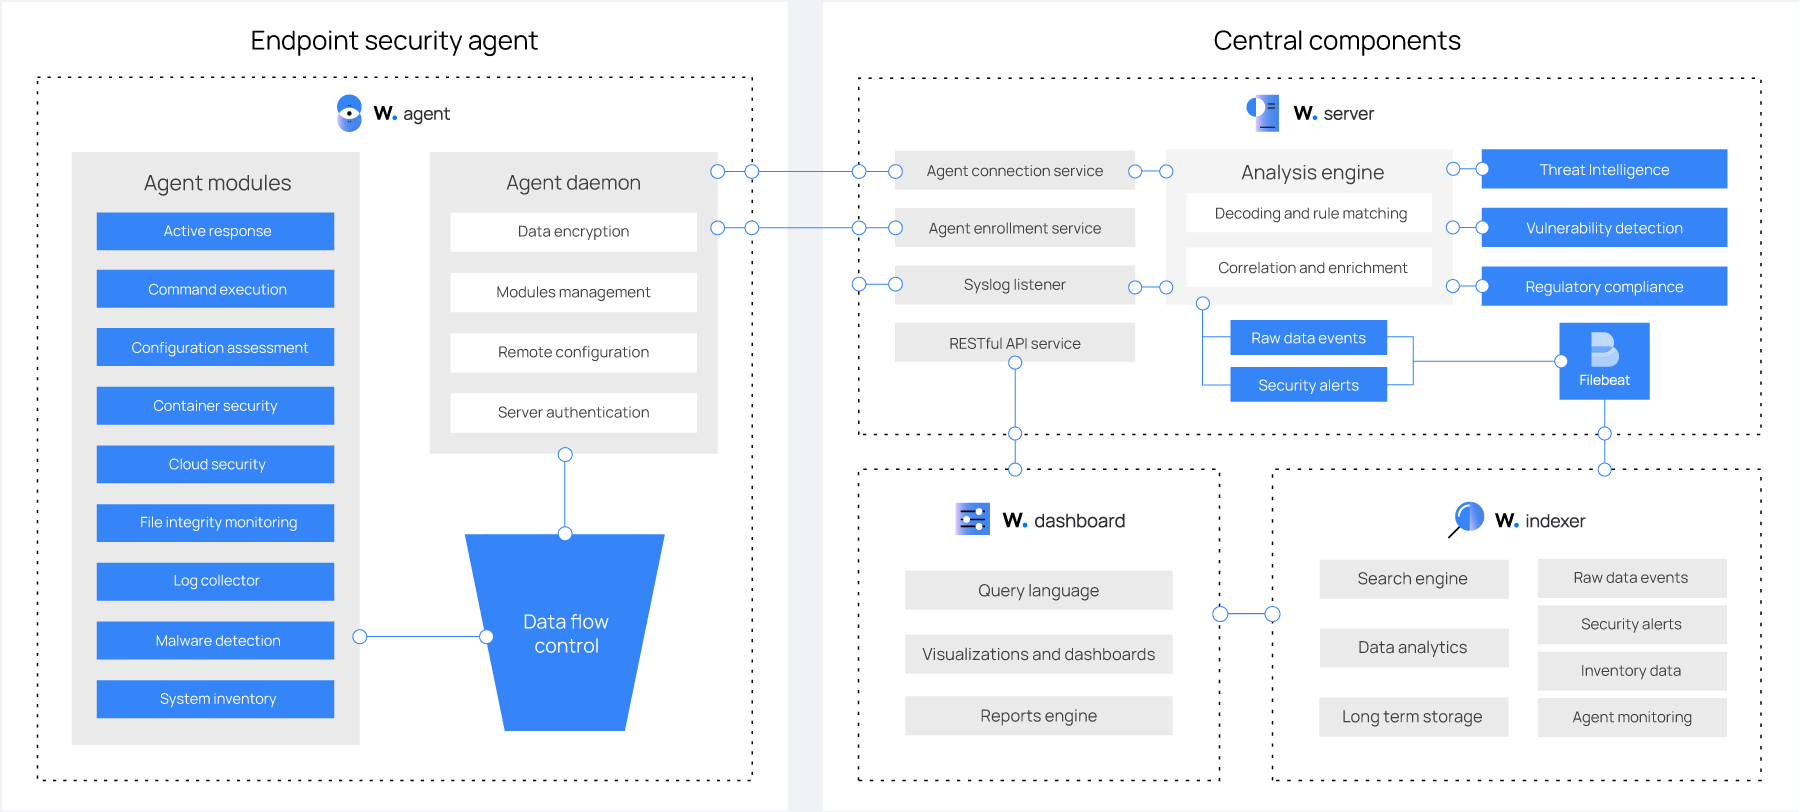
\includegraphics[width=1.0\textwidth]{figures/wazuh-components-and-data-flow1.png}
  \caption{Componentes de Wazuh}
  \label{fig:wazuh-components-and-data-flow}
\end{figure}

\section{Personal cualificado}
La plantilla de Wazuh está entre los 200 y 500 empleados a nivel mundial, entre ingenieros de software, ingenieros de seguridad (soporte técnico), ingenieros en Cloud, ingenieros de QA, desarrolladores de C/C++, diseñadores UX/UI, especialistas en DevOps y expertos en ciberseguridad \cite{linkedin_wazuh}.

\section{Dotación tecnológica}
Mi puesto consistía de un trabajo remoto, por tanto, no he recibido ninguna dotación tecnológica y he usado mi portátil para el trabajo. Se dispone de una oficina en Granada donde los empleados disponen de portátiles proporcionados por la propia empresa. Cabe destacar, que tienen clústeres de cómputo en la nube mediante servicios de AWS para poder realizar pruebas de entornos en la nube. La infraestructura de Wazuh se puede desplegar completamente en Amazon Web Services (AWS), haciendo uso de instancias EC2, almacenamiento en S3 y servicios de monitorización como CloudWatch para procesar y analizar datos de seguridad en tiempo real \cite{wazuh_agent_installation}. AWS es una plataforma de computación en la nube que ofrece más de 200 servicios que incluyen potencia de cómputo, opciones de almacenamiento, capacidad de red, etc.

Para la asignación de tareas se utiliza Jira. Esta plataforma de gestión de proyectos y seguimiento de actividades permite a los equipos planificar, monitorizar y administrar el desarrollo de software de manera eficiente.

Factorial es el software de gestión de recursos humanos que utiliza la empresa y se encarga de la organización del equipo, el horario del equipo donde cada miembro de Wazuh incluye su zona horaria y su turno en la pestaña de empleado. También cabe destacar que se usa para controlar las vacaciones, ausencias y todo lo relacionado a los derechos de cada trabajador.

Por último, para la comunicación y organización se usa la plataforma Slack, que es una plataforma parecida a Discord, Microsoft Teams, etc. La idea es que los empleados se puedan comunicar entre sí, además de ir anotando en tiempo real el trabajo que se está realizando. Esto último sirve a modo de seguimiento, donde cada empleado al final de su jornada tendrá que poner un resumen del mismo.